\documentclass[12pt]{article}
\usepackage[utf8]{inputenc}
\usepackage[T1]{fontenc}
\usepackage[francais]{babel}
\usepackage{microtype} % typography
\usepackage{csquotes}  % smart quotes
\usepackage{listings}
\usepackage{minted}
\usepackage{xcolor}
\usepackage{tcolorbox}
\usemintedstyle{monokai}
\usepackage[margin=1.5cm, top=3cm, bottom=1.5cm, headheight=15pt]{geometry}
\usepackage{fancyhdr}
\pagestyle{fancy}
\fancyhf{}
%\rhead{\textcolor{gray}{\small{19 avril 2023}}} 
\renewcommand{\headrulewidth}{0pt}
\cfoot{\thepage}
\renewcommand{\headrulewidth}{0pt}
\cfoot{\thepage}
\usepackage{titlesec}
\usepackage{hyperref}
\hypersetup{
    colorlinks=true,
    linkcolor=orange,
    urlcolor=orange
}
\usepackage{booktabs} % in preamble
\titleformat{\section}
{\normalfont\Large\bfseries\color{orange}}{\thesection}{1em}{}
\usepackage{enumitem}
\setlist{nosep}
\pagecolor{white} 
\color{black} 
\definecolor{bg}{rgb}{0.1, 0.14, 0.13} 
\setminted[kotlin]{bgcolor=bg} 
\usepackage{graphicx}
\usepackage{roboto}
\renewcommand{\familydefault}{\sfdefault}
\tcbuselibrary{listings, minted, skins}

\tcbset{listing engine=minted}

\newtcblisting{ktlst}{listing only, minted language=kotlin, minted style=paraiso-dark,
    colback=bg, enhanced, frame hidden, minted options={tabsize=2, breaklines, autogobble}}

% Fixed title and added empty author/date
\title{\textcolor{gray}{\Huge\bfseries KOTLIN POUR LES DÉBUTANTS}}
\author{}  % Added empty author to suppress warning
\date{}    % Suppress date
\usepackage{tabularx} % in preamble
\usepackage{tikz}
\usetikzlibrary{calc}
\usepackage[absolute,overlay]{textpos} 

\begin{document}
% Removed maketitle and kept only custom title page
\begin{titlepage}
\pagestyle{empty}
\newgeometry{margin=0cm, top=0cm, bottom=0cm, headheight=0pt}

\begin{tikzpicture}[remember picture,overlay]
  \node[inner sep=0pt] at (current page.center) {%
  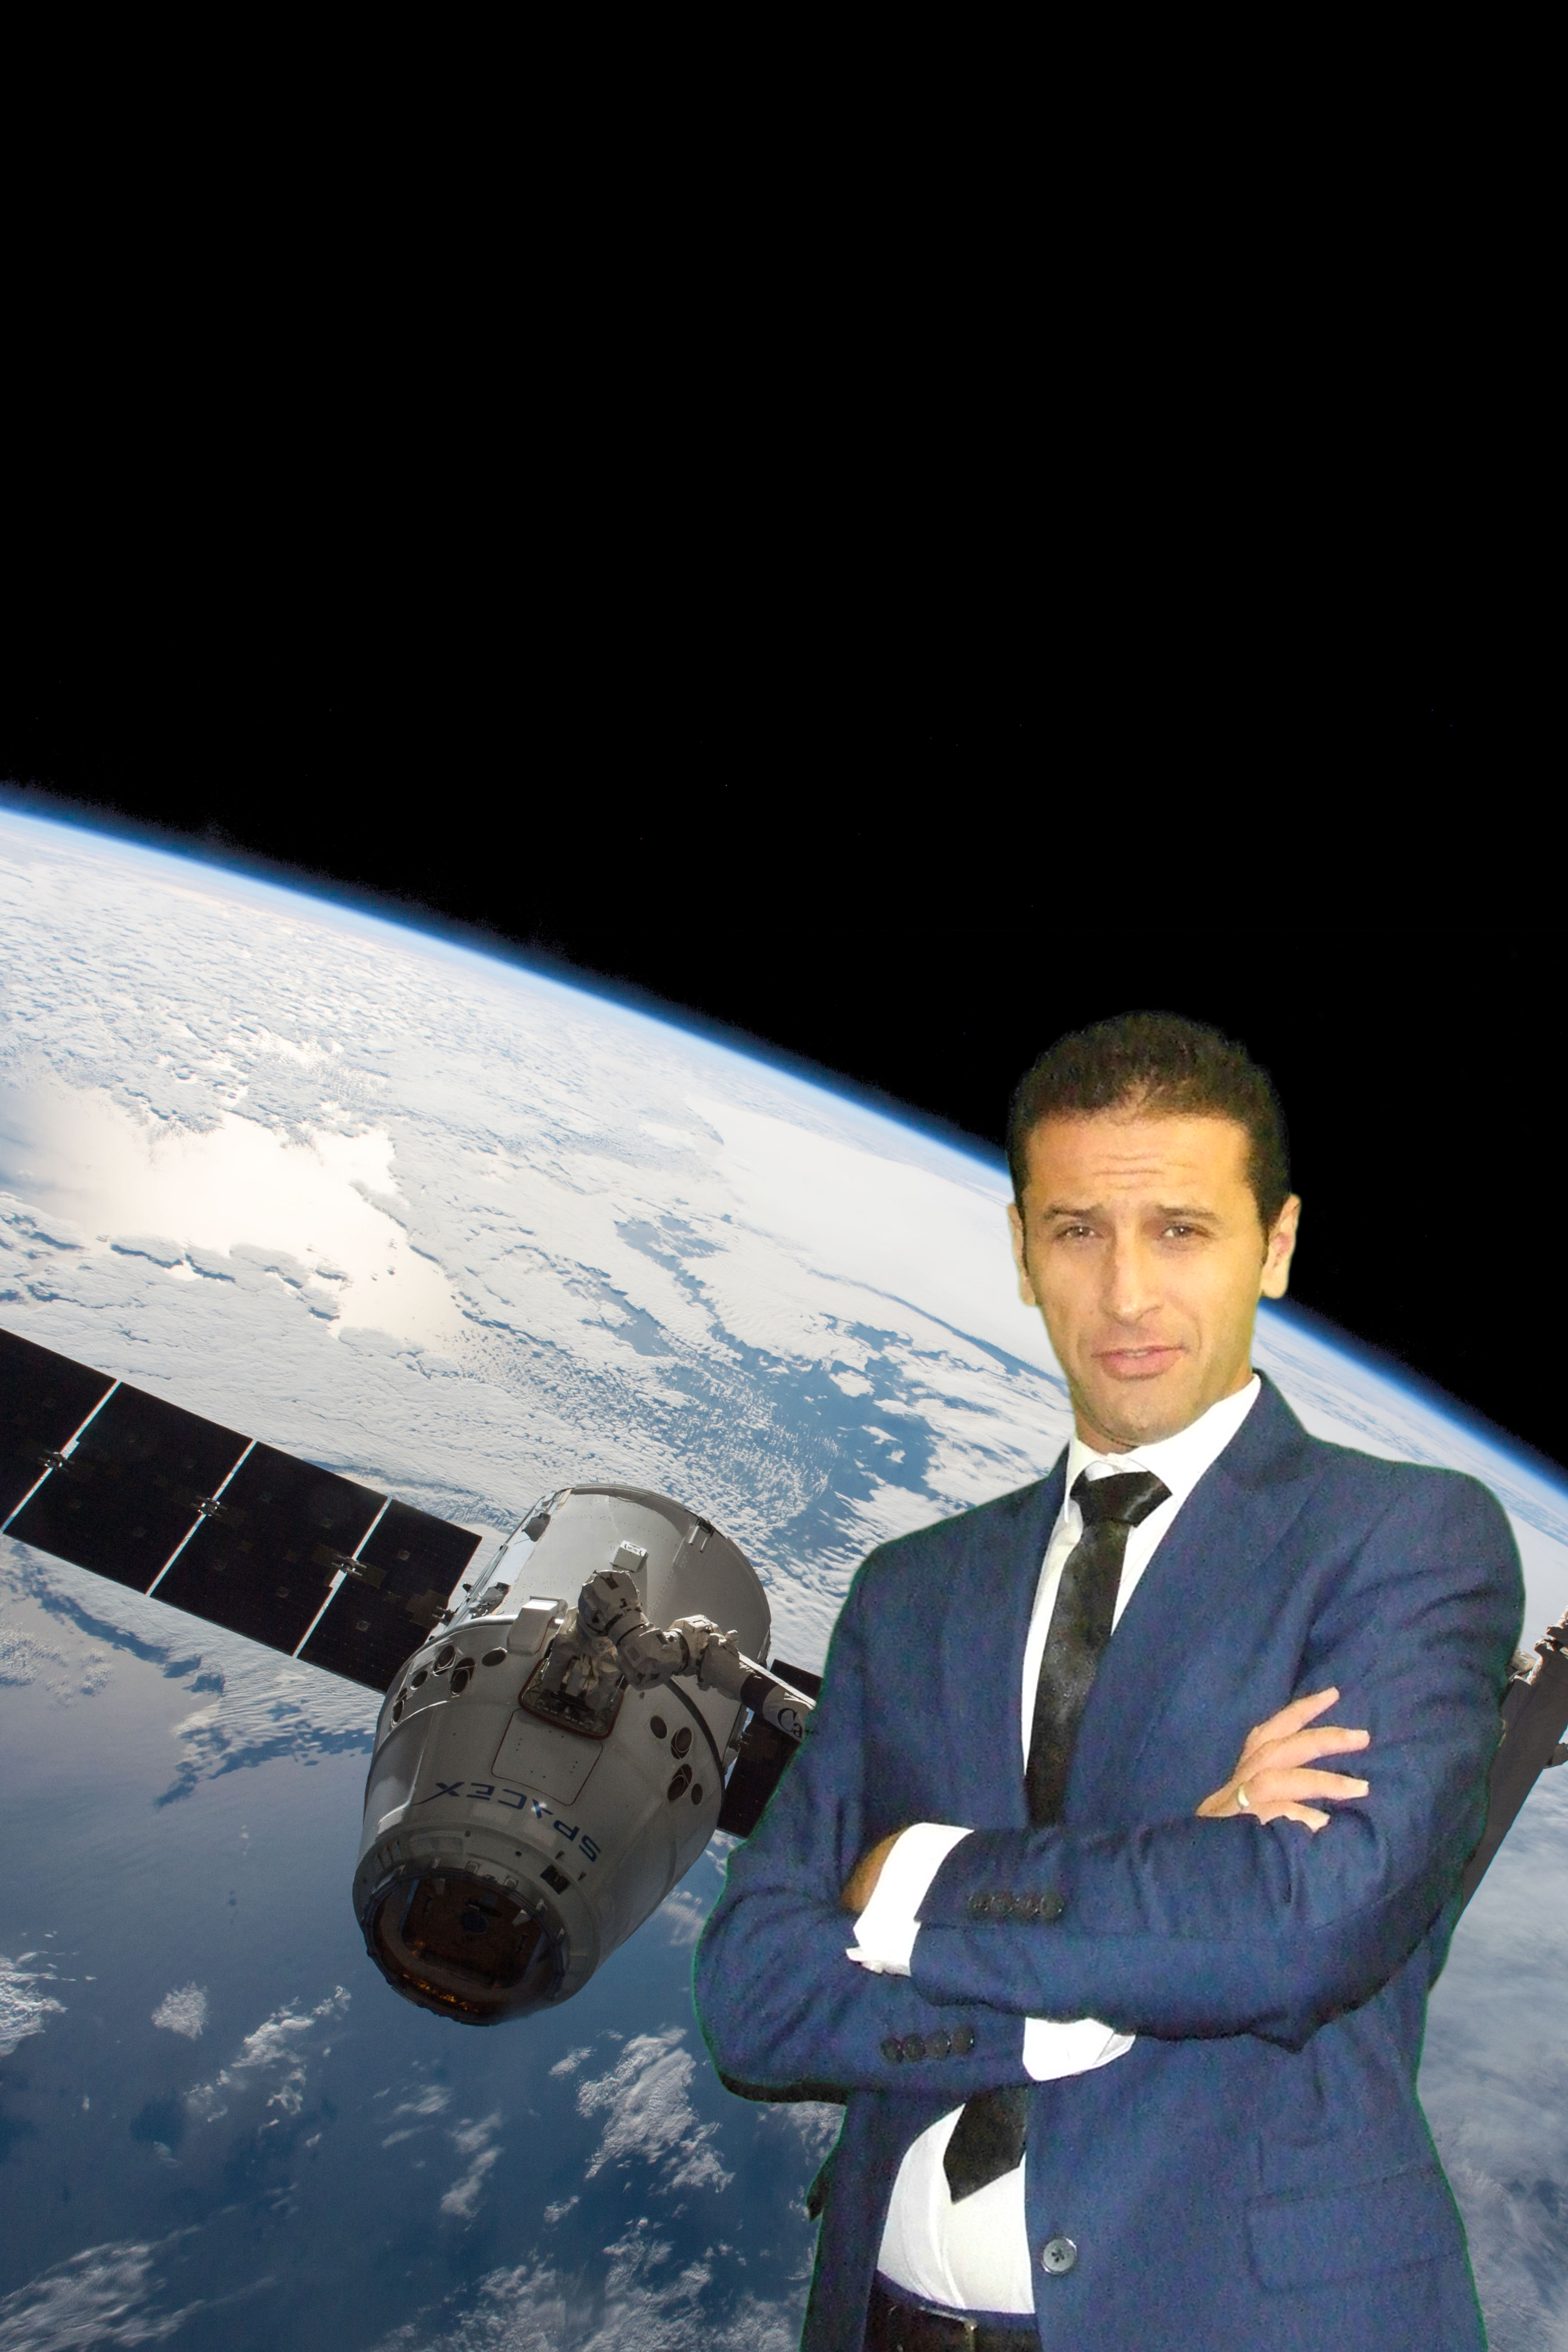
\includegraphics[width=\paperwidth, height=1.1\paperheight]{images/background.png}
  };

% --- Titre principal aligné à gauche ---
\node[inner sep=0pt, anchor=north, yshift=-2cm, align=left, xshift=-1cm] at (current page.north) {%

  \scalebox{3.9}{\textcolor{yellow}{\bfseries Développement}} 
  \\
  \\
  \scalebox{3.9}{\textcolor{yellow}{\bfseries d'applications mobiles}} 
  \\
  \\
  \scalebox{3.9}{\textcolor{yellow}{\bfseries modernes avec}} 
  \\
  \\
  \scalebox{3.9}{\textcolor{yellow}{\bfseries Jetpack et Kotlin}} 
};


% --- Sous-titre aligné à gauche ---
\node[inner sep=0pt, anchor=north, yshift=-20cm, align=left, xshift=-1cm] at (current page.north) {%
  \scalebox{2.5}{\textcolor{white}{\bfseries Construire}} 
  \\
  \\
  \scalebox{2.5}{\textcolor{white}{\bfseries des Applications Scalables}} 
  \\
  \\
  \scalebox{2.5}{\textcolor{white}{\bfseries avec Kotlin }} 
  \\
  \\
  \scalebox{2.5}{\textcolor{white}{\bfseries et une Architecture Propre}} 
};


\end{tikzpicture}

\restoregeometry 
\end{titlepage}



\newpage
% ----------------- Deuxième page de titre enrichie -----------------
\begin{titlepage}

% ======= CHOISIS UN FOND =======

% --- 1. Dégradé vertical ---
% --- Dégradé vertical + cercle décoratif ---
\begin{tikzpicture}[remember picture,overlay]
  % Dégradé de haut en bas
  \shade[top color=gray!10, bottom color=gray!40]
    (current page.north west) rectangle (current page.south east);

  % Cercle semi-transparent blanc par-dessus
  \fill[white, opacity=0.25] 
    ([xshift=6cm,yshift=-8cm]current page.north west) circle (10cm);
\end{tikzpicture}

% ======= CONTENU DE LA PAGE =======
\begin{flushleft}
\vspace*{-1.5cm} % marge réduite en haut

{\fontsize{38}{44}\selectfont \bfseries\textbf{
\begin{tabular}{l}
Développement \\
D'applications Mobiles \\
Modernes Avec \\
Jetpack Et Kotlin
\end{tabular}
}} \\[1.5cm]

{\large Améliorez vos applications en intégrant Jetpack et 
\\
en appliquant les concepts architecturaux modernes} \\[2cm]

{\Large \textbf{Touil Farouk}} \\[0.5cm]

{\large Développeur d’applications mobiles et concepteur
\\
 d’interfaces } \\[1.5cm]

% Photo
\includegraphics[width=5cm]{images/myphoto.png} \\[0.5cm]

{Email:  \texttt{farouktouil@hotmail.com, Alger }}\\[0.2cm]

\end{flushleft}
\end{titlepage}
% ----------------- End of Deuxième page de titre enrichie -----------------
\newpage



% Removed \maketitle here to prevent duplicate title page
\pagestyle{fancy}
\newpage
\section*{Sommaire}
\hypertarget{page:sommaire}{}  % <- la cible exacte du début du sommaire


{\footnotesize \textcolor{darkgray}{La navigation dans le sommaire et les chapitres est bidirectionnelle. }} 
{\footnotesize \textcolor{gray}{\textit{Chaque titre de section est cliquable et renvoie à la page correspondante. De même, chaque page de chapitre comporte un lien de retour vers le sommaire pour une navigation aisée.}}}

\begin{tabularx}{\textwidth}{@{}Xr@{}} % X = flexible column, r = right aligned
\textbf{Section} & \textbf{Page} \\
\addlinespace[0.5ex]

\multicolumn{2}{@{}l}{\footnotesize \textcolor{darkgray}{{Partie I : Les bases de Jetpack Compose}}} \\[0.5ex]
\hyperref[sec:intro]{Introduction : pourquoi Compose change tout} \dotfill & {\footnotesize \textcolor{darkgray}{{1}}} \\
\hyperref[sec:chapter-1]{Créer notre premier projet Compose} \dotfill & {\footnotesize \textcolor{darkgray}{{4}}}\\


\end{tabularx}



\newpage
\section{\hyperref[sec:summary]{\textcolor{orange}{Introduction à Kotlin}}}\label{sec:intro}

\textbf{Kotlin} est un langage moderne et concis conçu pour la JVM et largement utilisé pour le développement Android. Il améliore la productivité en réduisant le code boilerplate et en assurant une meilleure sécurité des types.

\section{\textcolor{orange}{Déclaration d'une classe en Kotlin}}\label{sec:classes}
\begin{ktlst}

[versions]
  hilt = "2.52"
  ksp = "2.0.21-1.0.25"

[libraries]
  hilt-android = { group = "com.google.dagger", name = "hilt-android", version.ref = "hilt" }
  hilt-compiler = { group = "com.google.dagger", name = "hilt-compiler", version.ref = "hilt" }
  hilt-navigation-compose = { group = "androidx.hilt", name = "hilt-navigation-compose", version = "1.2.0" }

[plugins]
  hilt-android = { id = "com.google.dagger.hilt.android", version.ref = "hilt" }
  ksp = { id = "com.google.devtools.ksp", version.ref = "ksp" }

\end{ktlst}

\section{\textcolor{orange}{Implémentation de MVVM en Android}}\label{sec:mvvm}
\begin{ktlst}
plugins {
    alias(libs.plugins.android.application) apply false
    alias(libs.plugins.kotlin.android) apply false
    alias(libs.plugins.kotlin.compose) apply false
    alias(libs.plugins.hilt.android) apply false   //  mark as apply false
    alias(libs.plugins.ksp) apply false           //  mark as apply false

}
\end{ktlst}

\begin{ktlst}
plugins {
    alias(libs.plugins.android.application)
    alias(libs.plugins.kotlin.android)
    alias(libs.plugins.kotlin.compose)
    //  apply Hilt + KSP only here
    alias(libs.plugins.hilt.android)
    alias(libs.plugins.ksp)
}
\end{ktlst}

\begin{ktlst}
dependencies {

    implementation(libs.androidx.core.ktx)
    implementation(libs.androidx.lifecycle.runtime.ktx)
    implementation(libs.androidx.activity.compose)
    implementation(platform(libs.androidx.compose.bom))
    implementation(libs.androidx.ui)
    implementation(libs.androidx.ui.graphics)
    implementation(libs.androidx.ui.tooling.preview)
    implementation(libs.androidx.material3)
    testImplementation(libs.junit)
    androidTestImplementation(libs.androidx.junit)
    androidTestImplementation(libs.androidx.espresso.core)
    androidTestImplementation(platform(libs.androidx.compose.bom))
    androidTestImplementation(libs.androidx.ui.test.junit4)
    debugImplementation(libs.androidx.ui.tooling)
    debugImplementation(libs.androidx.ui.test.manifest)

    implementation(libs.hilt.android)
    ksp(libs.hilt.compiler)
    implementation(libs.hilt.navigation.compose)
}
\end{ktlst}

\newpage
\section{\textcolor{orange}{Conclusion}}\label{sec:conclusion}
% --- HEADER ---
\fancyhead[L]{\small\href{https://developer.android.com}{Android Docs}}
\fancyhead[C]{\small\href{https://kotlinlang.org}{Kotlin Lang}}
\fancyhead[R]{\textcolor{gray}{\small{19 avril 2023}}}
L'utilisation de Kotlin pour le développement Android améliore l'efficacité et la sécurité du code tout en facilitant l'adoption d'architectures modernes comme MVVM. En adoptant Kotlin avec Clean Architecture, les développeurs peuvent créer des applications plus robustes et maintenables.

\begin{center}
\textbf{\textcolor{black}{Auteur: Touil Farouk}} \\  % Changed color to black
\textbf{\textcolor{black}{Email: farouktouil@hotmail.com}}
\end{center}
\fancyfoot[L]{\small\href{https://developer.android.com}{Android Docs}}
\fancyfoot[C]{\thepage}
\fancyfoot[R]{\small\href{https://kotlinlang.org}{Kotlin Lang}}

\end{document}